% This section describes the design of the memory system model. How host target
% decoupling is achieved. What configurations are available.

Our memory system model \textit{generator} describes a space of individual
\textit{instances} that model different memory systems. Implemented in
Chisel\cite{Chisel}, the generator emits Verilog that can be integrated into
larger FPGA projects. All instances are runtime-configurable via memory-mapped registers.

\subsection{Interfaces}

All instances of the model have three interfaces. Each interface implements the AXI4 standard:

\begin{enumerate} \item \textbf{Target-Side} (Host-decoupled AXI4 slave with sync. reset). This
is the target's view of the memory system, and timing tokens are used to synchronize time between the processor and the modeled memory system. As a host-decoupled interface, it consumes a single input token and produces a single output token for each target cycle of execution (see Section \ref{sec:infrastructure} for details). 

    \item \textbf{Host-Side} (AXI4 master). This interface is used by the model to access the FPGA host's memory, which contains the actual data backing the simulated memory system. It runs independently of target time.

    \item \textbf{Configuration-Side} (AXI4-lite slave). This exposes
        memory-mapped configuration registers to the simulation driver running on the host. This allows reconfiguring the memory model at runtime.
\end{enumerate}

We selected AXI4 as the default interface as it is the most common memory
interface presented by FPGA IP and widely implemented in ASICs. Both major FPGA
vendors provide IP to bridge AXI4 to other standards, as well as adapters, to
connect master and slave devices that may have different interface widths. We expect
this to facilitate adoption. 

%In general, the widths of all fields in target-side and host-side interfaces
%are expected to match, with the exception of ARID and AWID. Here, the model can
%optionally reduce on the host-side ID width to the specification's recommended of
%maximum 4 bits or tie it off altogether, to prevent host-memory system
%reorderings.

\begin{figure}
	\centering
	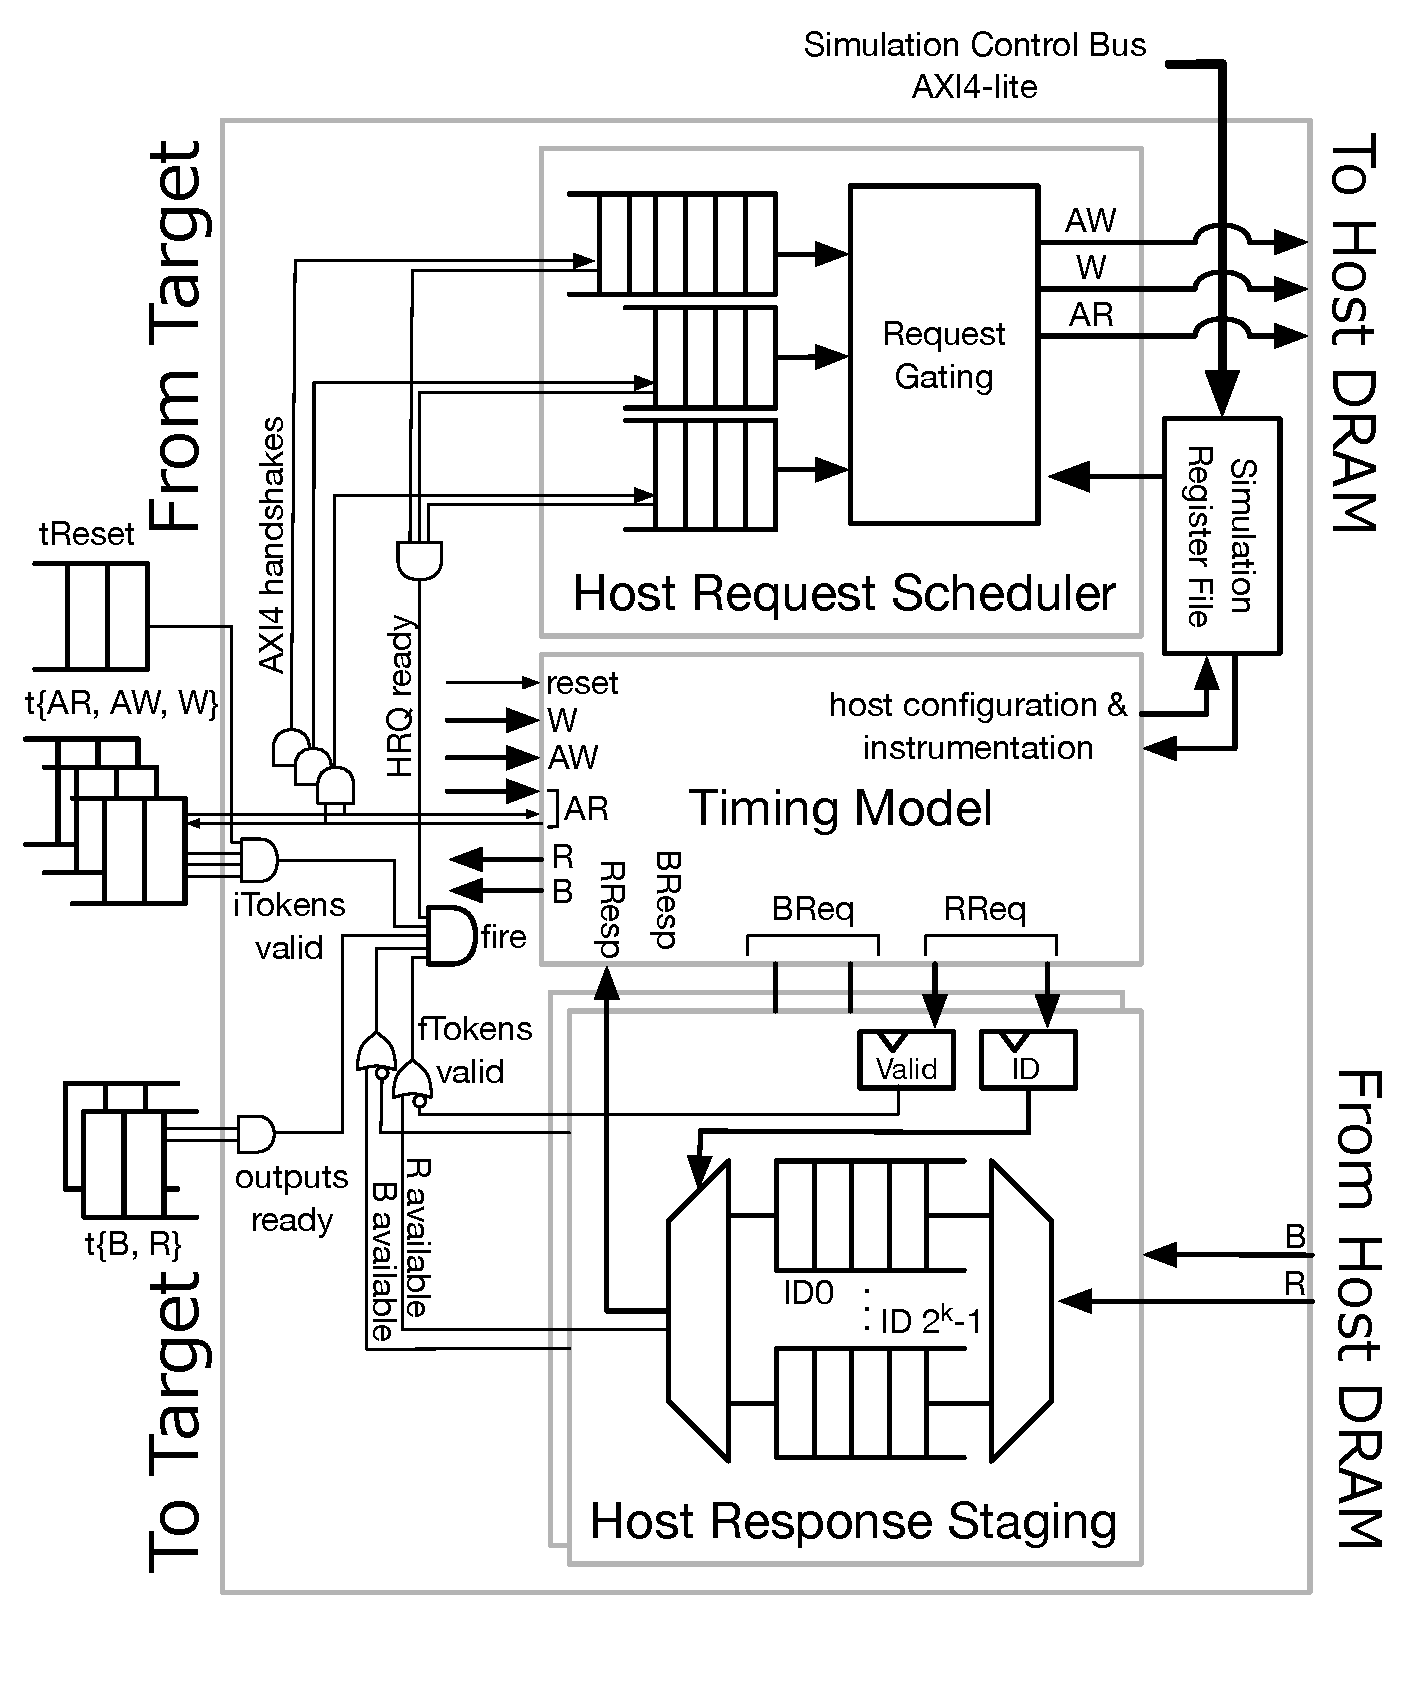
\includegraphics[width=\columnwidth]{figures/memory-model-block-diagram.pdf}
	\caption{Top-level diagram of memory system model with latency-bandwidth pipe timing model}
	\label{fig:timing_model}
\end{figure}

\subsection{Operation}

%A given instance uses the memory system of the FPGA-host as a backing store for
%the functional model of the target memory system. It forwards translated
%requests from the target to the host and buffers the responses. In parallel,
%the timing model determines on which target cycle it should release responses
%and accept new requests. If the host memory system is too fast, the responses
%are buffered until the appropriate target cycle. If it is too slow, the model
%stalls the target until the response from the host memory system has been
%received.

Figure~\ref{fig:timing_model} represents an instance of the memory system
model. The \textit{ingress} unit accepts requests from the target memory
interface and fowards them to the host memory system (with some address translation).
In parallel, the timing model determines on which target cycle it should
release responses and accept new requests. Responses from the host memory
system are buffered in the \textit{egress} unit until the timing model
determines is the correct cycle to release them. If the host memory system is
too slow, the timing model stalls the target until the response from the host
memory system has been received.

\subsubsection{Functional-Timing Split}

Our memory system model employs a functional-timing split. This relies on the
target design being host-target decoupled as described in
Section~\ref{sec:host-target-decoupling}. We refer to a the set of target
signals present on a target interface in a given target cycle as a timing
\textit{token}. Figure~\ref{fig:model_operation} illustrates this split with
red indicating timing tokens and blue indicating functional memory operations.

The functional ``model'' portion consists of the ingress unit, egress unit and
the AXI-4 memory slave configuration port. The ingress unit aggregates tokens
from the target into complete requests before forwarding them to the host
memory system. The egress unit collects responses from the host memory system
and buffers them until they are requested by the \textit{timing model}. While
the AXI4 slave is often just a DRAM controller on the FPGA host, it could also be a
device that uses local FPGA DRAM as cache for a larger store (see
LEAP\cite{leapscratchpad}).

In parallel, the timing model consumes the input token and generates a new
output token for every target cycle of execution. Each output token represents
the value of all signals that would be driven by the memory controller
(backpressure on request channels, and the payload and valid bits of response
channels) after they have ``settled'' for that cycle. In order to populate a
token with valid data, the timing model fetches the corresponding data from the
egress unit using channel ID as the key.

\begin{figure*}
	\centering
	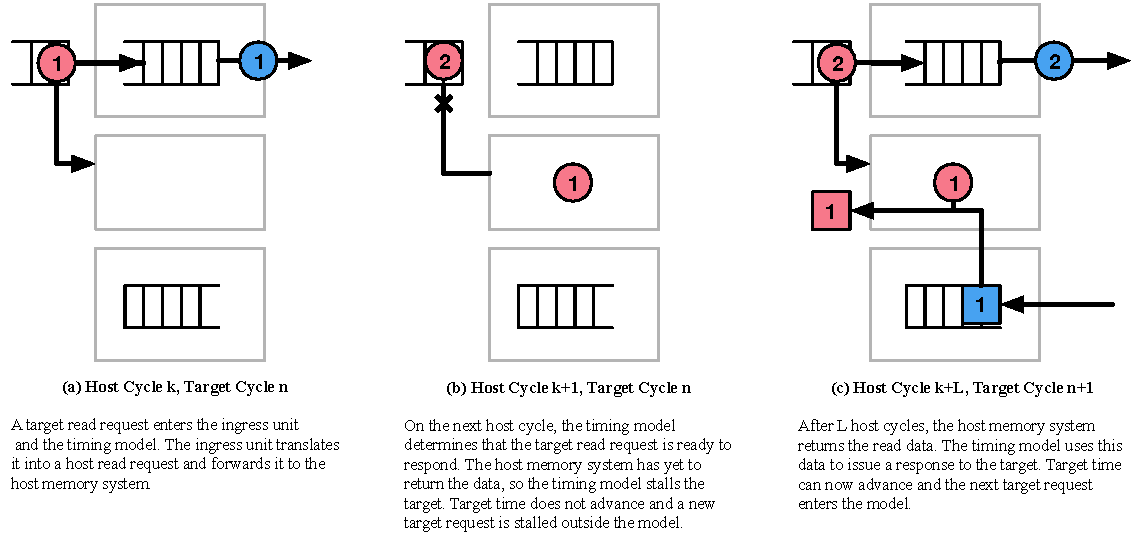
\includegraphics[width=0.8\textwidth]{figures/memory-model-operation.pdf}
	\caption{Operation of a single-cycle "magic" memory}
	\label{fig:model_operation}
\end{figure*}

\subsubsection{Egress Unit Design}\label{egress}
Since both the host memory system and the timing model may reorder responses
(as permitted by AXI4 specification), the egress unit implements a set of
virtual queues for each AXI4 channel. Each queue represents the FIFO ordering
within a single channel ID. The implementation of the virtual queues differs
based on:

\begin{itemize}
    \item Maximum number of outstanding requests
    \item Maximum number of AXI channels in use
    \item Minimum and maximum read request length
\end{itemize}

For a small number of IDs or a small number of outstanding requests, the
memory system model implements each virtual queue as a physical queue co-located in
the same BRAM. For greater numbers of AXI IDs, it dynamically assigns entries
within the block RAM to each response and maintains a list of pointers to those
entries for each channel ID.

\subsection{Timing Model Classes}
\label{sec:timing_model}

We provide four base timing model classes:

\begin{itemize}
    \item \textbf{Latency-Bandwidth Pipe} Applies independently programmable
    latencies to read and write requests. The pipe does not accept any new requests beyond
    a programmable limit. This serves as a coarse-grain bandwidth bound via
    Little's law.

    \item \textbf{Bank Conflict} Adds a penalty of $max(0, t_{CP} -
    t_{\Delta})$ to a base latency if a read or write request used the bank
    $t_{\Delta}$ cycles prior, where $t_{CP}$ is the maximum conflict penalty.

    \item \textbf{FCFS DRAM MAS} Implements \ref{fcfs} with configurable open and closed page policy.
    \item \textbf{FR-FCFS DRAM MAS} Implements \ref{frfcfs} with an open page policy.
\end{itemize}


Note that while the latter two models do have programmable $t_{RP}$, $t_{CS}$,
$t_{RCD}$, they are incomplete models of a generic DDR DRAM. For example, they
do not check against all DRAM timing constraints, nor do they model refresh.
They do, however, significantly improve modeling fidelity of DRAM memory systems
(with their respective MASs). We
expect that the latency-bandwidth pipe and bank conflict model will also
suffice for modeling a slew of other memory technologies to a first-order approximation.

\subsection{Configurability}

There are two points at which the model can be configured.  At
\textit{generation time}, the designer selects an appropriate instance. At
\textit{simulation time}, the instance is programmed through its
configuration-side interface to further set its behavior. Simulation time
configurability permits the designer to perform parameter sweeps without
needing to recompile the simulator bitstream -- at the expense of FPGA
resources. Since both timing and functional components of an instance are
provisioned pessimistically, giving hints to generator can greatly reduce FPGA
resource utilization. We outline some programmability-area tradeoffs here.

\begin{itemize}
    \item \textbf{Reducing functional component size.} The simulation designer can call
out constraints on the behavior of the AXI masters to reduce the size of the
ingress and egress units. This achieved by putting bounds on the parameters
defined in \ref{egress}.

	\item \textbf{Selecting the timing model class.} Simpler timing models consume fewer resources.

	\item \textbf{Reducing model programmability.} By default, each timing model class
exposes all of its parameters as programmable registers on the simulation
memory map. The generator permits tying particular knobs to static values,
saving FPGA resources. For example, the bank-conflict model has a runtime
configurable number of banks. Specifying a fixed number of banks at generation
time removes the unneeded programmable registers and bank state.

	\item \textbf{Reducing model instrumentation.} Model instances can be generated with
instrumentation to track specific events and capture activity traces. This
instrumentation is exposed on the simulation memory map. Generating the model
with less instrumentation uses fewer resources.
\end{itemize}
